\documentclass[]{article}
\usepackage{lmodern}
\usepackage{amssymb,amsmath}
\usepackage{ifxetex,ifluatex}
\usepackage{fixltx2e} % provides \textsubscript
\ifnum 0\ifxetex 1\fi\ifluatex 1\fi=0 % if pdftex
  \usepackage[T1]{fontenc}
  \usepackage[utf8]{inputenc}
\else % if luatex or xelatex
  \ifxetex
    \usepackage{mathspec}
  \else
    \usepackage{fontspec}
  \fi
  \defaultfontfeatures{Ligatures=TeX,Scale=MatchLowercase}
\fi
% use upquote if available, for straight quotes in verbatim environments
\IfFileExists{upquote.sty}{\usepackage{upquote}}{}
% use microtype if available
\IfFileExists{microtype.sty}{%
\usepackage{microtype}
\UseMicrotypeSet[protrusion]{basicmath} % disable protrusion for tt fonts
}{}
\usepackage[margin=1in]{geometry}
\usepackage{hyperref}
\hypersetup{unicode=true,
            pdftitle={Empirical calibration of p-values},
            pdfauthor={Martijn J. Schuemie, Marc A. Suchard},
            pdfborder={0 0 0},
            breaklinks=true}
\urlstyle{same}  % don't use monospace font for urls
\usepackage{color}
\usepackage{fancyvrb}
\newcommand{\VerbBar}{|}
\newcommand{\VERB}{\Verb[commandchars=\\\{\}]}
\DefineVerbatimEnvironment{Highlighting}{Verbatim}{commandchars=\\\{\}}
% Add ',fontsize=\small' for more characters per line
\usepackage{framed}
\definecolor{shadecolor}{RGB}{248,248,248}
\newenvironment{Shaded}{\begin{snugshade}}{\end{snugshade}}
\newcommand{\AlertTok}[1]{\textcolor[rgb]{0.94,0.16,0.16}{#1}}
\newcommand{\AnnotationTok}[1]{\textcolor[rgb]{0.56,0.35,0.01}{\textbf{\textit{#1}}}}
\newcommand{\AttributeTok}[1]{\textcolor[rgb]{0.77,0.63,0.00}{#1}}
\newcommand{\BaseNTok}[1]{\textcolor[rgb]{0.00,0.00,0.81}{#1}}
\newcommand{\BuiltInTok}[1]{#1}
\newcommand{\CharTok}[1]{\textcolor[rgb]{0.31,0.60,0.02}{#1}}
\newcommand{\CommentTok}[1]{\textcolor[rgb]{0.56,0.35,0.01}{\textit{#1}}}
\newcommand{\CommentVarTok}[1]{\textcolor[rgb]{0.56,0.35,0.01}{\textbf{\textit{#1}}}}
\newcommand{\ConstantTok}[1]{\textcolor[rgb]{0.00,0.00,0.00}{#1}}
\newcommand{\ControlFlowTok}[1]{\textcolor[rgb]{0.13,0.29,0.53}{\textbf{#1}}}
\newcommand{\DataTypeTok}[1]{\textcolor[rgb]{0.13,0.29,0.53}{#1}}
\newcommand{\DecValTok}[1]{\textcolor[rgb]{0.00,0.00,0.81}{#1}}
\newcommand{\DocumentationTok}[1]{\textcolor[rgb]{0.56,0.35,0.01}{\textbf{\textit{#1}}}}
\newcommand{\ErrorTok}[1]{\textcolor[rgb]{0.64,0.00,0.00}{\textbf{#1}}}
\newcommand{\ExtensionTok}[1]{#1}
\newcommand{\FloatTok}[1]{\textcolor[rgb]{0.00,0.00,0.81}{#1}}
\newcommand{\FunctionTok}[1]{\textcolor[rgb]{0.00,0.00,0.00}{#1}}
\newcommand{\ImportTok}[1]{#1}
\newcommand{\InformationTok}[1]{\textcolor[rgb]{0.56,0.35,0.01}{\textbf{\textit{#1}}}}
\newcommand{\KeywordTok}[1]{\textcolor[rgb]{0.13,0.29,0.53}{\textbf{#1}}}
\newcommand{\NormalTok}[1]{#1}
\newcommand{\OperatorTok}[1]{\textcolor[rgb]{0.81,0.36,0.00}{\textbf{#1}}}
\newcommand{\OtherTok}[1]{\textcolor[rgb]{0.56,0.35,0.01}{#1}}
\newcommand{\PreprocessorTok}[1]{\textcolor[rgb]{0.56,0.35,0.01}{\textit{#1}}}
\newcommand{\RegionMarkerTok}[1]{#1}
\newcommand{\SpecialCharTok}[1]{\textcolor[rgb]{0.00,0.00,0.00}{#1}}
\newcommand{\SpecialStringTok}[1]{\textcolor[rgb]{0.31,0.60,0.02}{#1}}
\newcommand{\StringTok}[1]{\textcolor[rgb]{0.31,0.60,0.02}{#1}}
\newcommand{\VariableTok}[1]{\textcolor[rgb]{0.00,0.00,0.00}{#1}}
\newcommand{\VerbatimStringTok}[1]{\textcolor[rgb]{0.31,0.60,0.02}{#1}}
\newcommand{\WarningTok}[1]{\textcolor[rgb]{0.56,0.35,0.01}{\textbf{\textit{#1}}}}
\usepackage{graphicx,grffile}
\makeatletter
\def\maxwidth{\ifdim\Gin@nat@width>\linewidth\linewidth\else\Gin@nat@width\fi}
\def\maxheight{\ifdim\Gin@nat@height>\textheight\textheight\else\Gin@nat@height\fi}
\makeatother
% Scale images if necessary, so that they will not overflow the page
% margins by default, and it is still possible to overwrite the defaults
% using explicit options in \includegraphics[width, height, ...]{}
\setkeys{Gin}{width=\maxwidth,height=\maxheight,keepaspectratio}
\IfFileExists{parskip.sty}{%
\usepackage{parskip}
}{% else
\setlength{\parindent}{0pt}
\setlength{\parskip}{6pt plus 2pt minus 1pt}
}
\setlength{\emergencystretch}{3em}  % prevent overfull lines
\providecommand{\tightlist}{%
  \setlength{\itemsep}{0pt}\setlength{\parskip}{0pt}}
\setcounter{secnumdepth}{5}
% Redefines (sub)paragraphs to behave more like sections
\ifx\paragraph\undefined\else
\let\oldparagraph\paragraph
\renewcommand{\paragraph}[1]{\oldparagraph{#1}\mbox{}}
\fi
\ifx\subparagraph\undefined\else
\let\oldsubparagraph\subparagraph
\renewcommand{\subparagraph}[1]{\oldsubparagraph{#1}\mbox{}}
\fi

%%% Use protect on footnotes to avoid problems with footnotes in titles
\let\rmarkdownfootnote\footnote%
\def\footnote{\protect\rmarkdownfootnote}

%%% Change title format to be more compact
\usepackage{titling}

% Create subtitle command for use in maketitle
\newcommand{\subtitle}[1]{
  \posttitle{
    \begin{center}\large#1\end{center}
    }
}

\setlength{\droptitle}{-2em}

  \title{Empirical calibration of p-values}
    \pretitle{\vspace{\droptitle}\centering\huge}
  \posttitle{\par}
    \author{Martijn J. Schuemie, Marc A. Suchard}
    \preauthor{\centering\large\emph}
  \postauthor{\par}
      \predate{\centering\large\emph}
  \postdate{\par}
    \date{2019-05-07}


\begin{document}
\maketitle

{
\setcounter{tocdepth}{2}
\tableofcontents
}
\hypertarget{introduction}{%
\section{Introduction}\label{introduction}}

In observational studies, there is always the possibility that an effect
size estimate is biased. This can be true even for advanced, well
thought out study designs, because of unmeasured or unmodeled
confounding. Negative controls (test-hypotheses where the exposure is
not believed to cause the outcome) can be used to detect the potential
for bias in a study, and with enough negative controls we can start to
estimate the systematic error distribution inherent in an observational
analysis. We can then use this estimated distribution to compute a
calibrated p-value, which reflects the probability of observing an
effect size estimate when the null hypothesis (of no effect) is true,
taking both systematic and random error into account.

In this document we will use an example study to illustrate how this can
be done using the \texttt{EmpiricalCalibration} R package. In the
example, we will try to answer the question whether sertraline (an SSRI)
causes GI bleeding. We use a Self-Controlled Case Series (SCCS) design,
and have applied this to a large insurance claims database.

The results from this study are available in the package, and can be
loaded using the \texttt{data()} command:

\begin{Shaded}
\begin{Highlighting}[]
\KeywordTok{data}\NormalTok{(sccs)}
\NormalTok{drugOfInterest <-}\StringTok{ }\NormalTok{sccs[sccs}\OperatorTok{$}\NormalTok{groundTruth }\OperatorTok{==}\StringTok{ }\DecValTok{1}\NormalTok{, ]}
\NormalTok{drugOfInterest}
\end{Highlighting}
\end{Shaded}

\begin{verbatim}
##     drugName groundTruth     logRr    seLogRr
## 6 Sertraline           1 0.7326235 0.07371708
\end{verbatim}

\begin{Shaded}
\begin{Highlighting}[]
\KeywordTok{exp}\NormalTok{(drugOfInterest}\OperatorTok{$}\NormalTok{logRr)}
\end{Highlighting}
\end{Shaded}

\begin{verbatim}
## [1] 2.080532
\end{verbatim}

\begin{Shaded}
\begin{Highlighting}[]
\KeywordTok{computeTraditionalP}\NormalTok{(drugOfInterest}\OperatorTok{$}\NormalTok{logRr, drugOfInterest}\OperatorTok{$}\NormalTok{seLogRr)}
\end{Highlighting}
\end{Shaded}

\begin{verbatim}
## [1] 0
\end{verbatim}

Here we see that the effect estimate for sertraline is 2.1, with a
p-value that is so small R rounds it to 0.

\hypertarget{negative-controls}{%
\section{Negative controls}\label{negative-controls}}

Negative controls are drug-outcome pairs where we believe the drug does
not cause (or prevent) the outcome. In other words, we believe the true
effect size to be a relative risk of 1. We would prefer our negative
controls to have some resemblance with out hypothesis of interest (in
our example sertraline - GI bleed), and we therefore typically pick
negative controls where the outcome is the same (exposure controls), or
the exposure is the same (outcome controls). In this example, we have
opted for exposure controls, and have identified a set of drugs not
believed to cause GI bleed. We have executed exactly the same analysis
for these exposures, resulting in a set of effect size estimates, one
per negative control:

\begin{Shaded}
\begin{Highlighting}[]
\KeywordTok{data}\NormalTok{(sccs)}
\NormalTok{negatives <-}\StringTok{ }\NormalTok{sccs[sccs}\OperatorTok{$}\NormalTok{groundTruth }\OperatorTok{==}\StringTok{ }\DecValTok{0}\NormalTok{, ]}
\KeywordTok{head}\NormalTok{(negatives)}
\end{Highlighting}
\end{Shaded}

\begin{verbatim}
##           drugName groundTruth     logRr   seLogRr
## 1      Thiothixene           0 0.4339021 0.7617538
## 2    Methocarbamol           0 0.6363184 0.1839892
## 4      Phentermine           0 0.9297549 0.2979802
## 5       Disulfiram           0 1.6919273 0.5955222
## 7         Orlistat           0 0.5261691 0.1967199
## 8 Prochlorperazine           0 0.8581890 0.1308460
\end{verbatim}

\hypertarget{plot-negative-control-effect-sizes}{%
\subsection{Plot negative control effect
sizes}\label{plot-negative-control-effect-sizes}}

We can start by creating a forest plot of our negative controls:

\begin{Shaded}
\begin{Highlighting}[]
\KeywordTok{plotForest}\NormalTok{(negatives}\OperatorTok{$}\NormalTok{logRr, negatives}\OperatorTok{$}\NormalTok{seLogRr, negatives}\OperatorTok{$}\NormalTok{drugName)}
\end{Highlighting}
\end{Shaded}

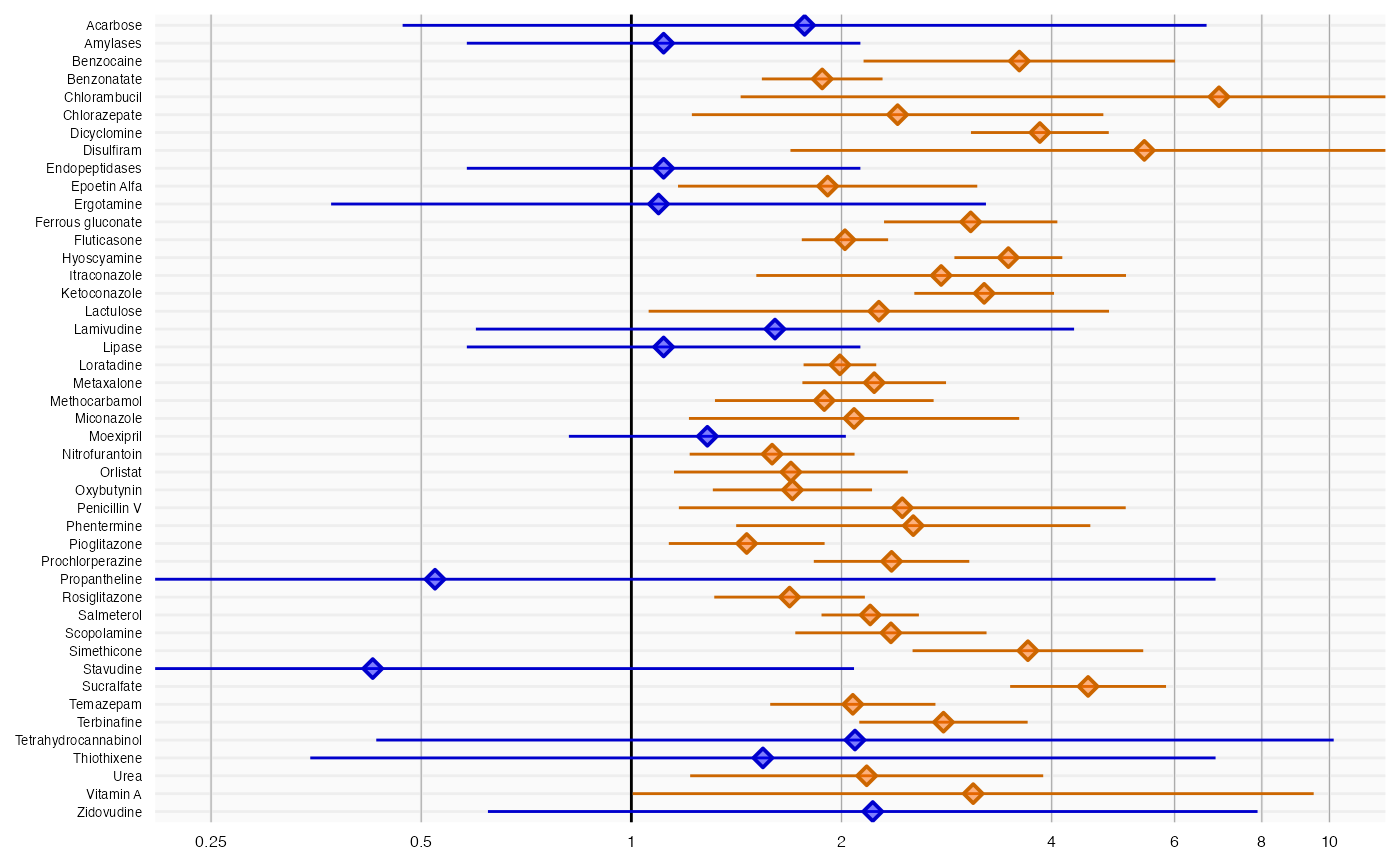
\includegraphics{../inst/doc/EmpiricalPCalibrationVignette_files/figure-latex/unnamed-chunk-4-1.pdf}

Here we see that many negative controls have a confidence interval that
does not include a relative risk of 1 (orange lines), certainly more
than the expected 5\%. This indicates the analysis has systematic error.

\hypertarget{empirical-null-distribution}{%
\section{Empirical null
distribution}\label{empirical-null-distribution}}

\hypertarget{fitting-the-null-distribution}{%
\subsection{Fitting the null
distribution}\label{fitting-the-null-distribution}}

We can use the negative controls to estimate the systematic error
distribution. We assume the distribution is a Gaussian distribution,
which we have found to give good performance in the past.

\begin{Shaded}
\begin{Highlighting}[]
\NormalTok{null <-}\StringTok{ }\KeywordTok{fitNull}\NormalTok{(negatives}\OperatorTok{$}\NormalTok{logRr, negatives}\OperatorTok{$}\NormalTok{seLogRr)}
\NormalTok{null}
\end{Highlighting}
\end{Shaded}

\begin{verbatim}
## Estimated null distribution
## 
##      Estimate
## Mean   0.7921
## SD     0.2834
\end{verbatim}

We see that the mean of our distribution is greater than 0, indicating
the analysis is positively biased. We also see the standard deviation is
greater than 0.25, indicating there is considerable variability in the
systematic error from one estimate to the next.

\hypertarget{evaluating-the-calibration}{%
\subsection{Evaluating the
calibration}\label{evaluating-the-calibration}}

To evaluate whether our estimation of the systematic error distribution
is a good one, we can test whether the calibrated p-value is truly
calibrated, meaning the fraction of negative controls with a p-value
below alpha is approximately the same as alpha:

\begin{Shaded}
\begin{Highlighting}[]
\KeywordTok{plotCalibration}\NormalTok{(negatives}\OperatorTok{$}\NormalTok{logRr,negatives}\OperatorTok{$}\NormalTok{seLogRr)}
\end{Highlighting}
\end{Shaded}

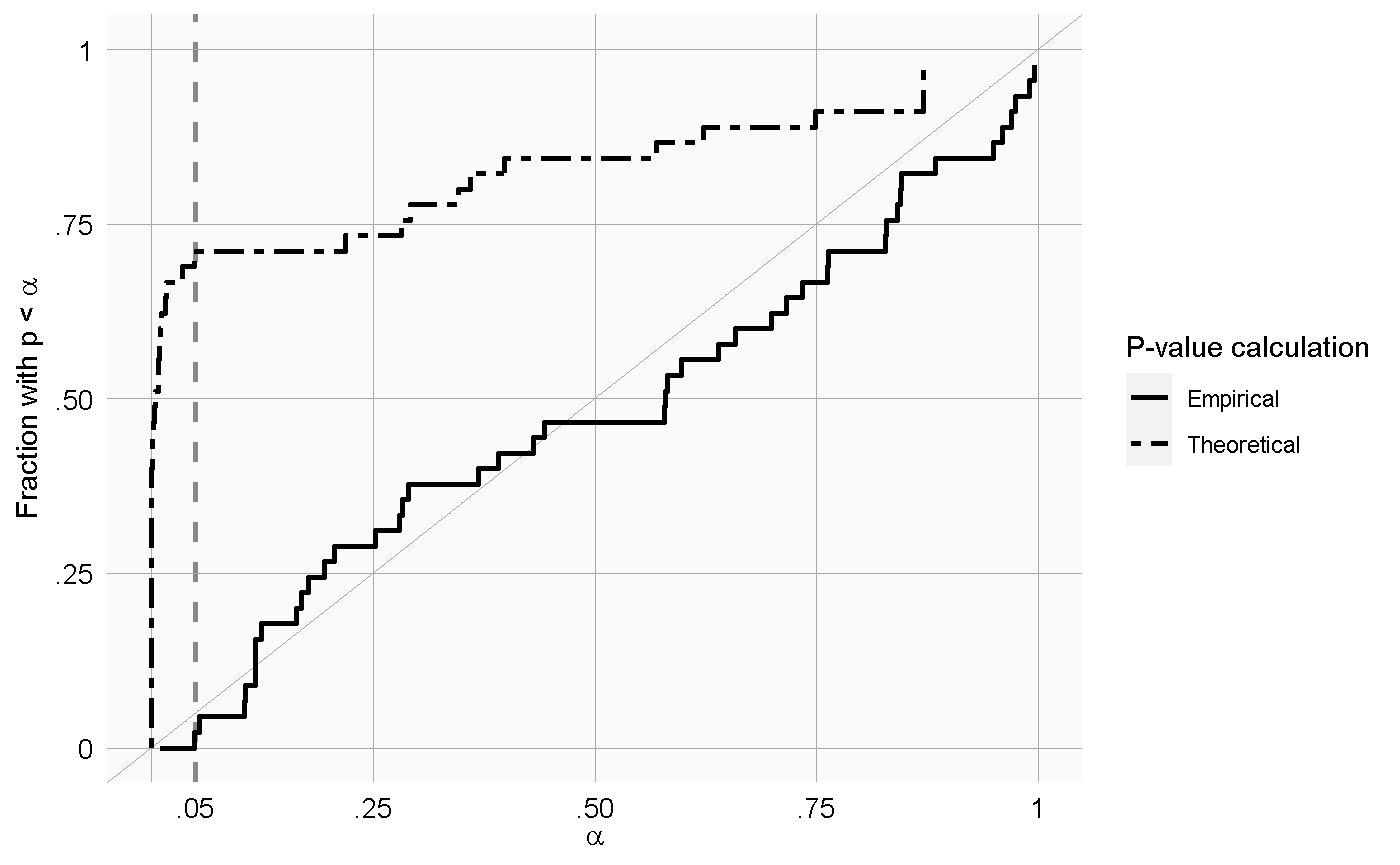
\includegraphics{../inst/doc/EmpiricalPCalibrationVignette_files/figure-latex/unnamed-chunk-6-1.pdf}

This method uses a leave-one-out design: for every negative control, the
null distribution is fitted using all other negative controls, and the
calibrated p-value for that negative control is computed.

In the graph we see that the calibrated p-value is much closer to the
diagonal than the uncalibrated p-value.

\hypertarget{plotting-the-null-distribution}{%
\subsection{Plotting the null
distribution}\label{plotting-the-null-distribution}}

We can create a graphical representation of the null distribution,
together with the negative controls used to estimate that distribution:

\begin{Shaded}
\begin{Highlighting}[]
\KeywordTok{plotCalibrationEffect}\NormalTok{(negatives}\OperatorTok{$}\NormalTok{logRr,negatives}\OperatorTok{$}\NormalTok{seLogRr, }\DataTypeTok{null =}\NormalTok{ null)}
\end{Highlighting}
\end{Shaded}

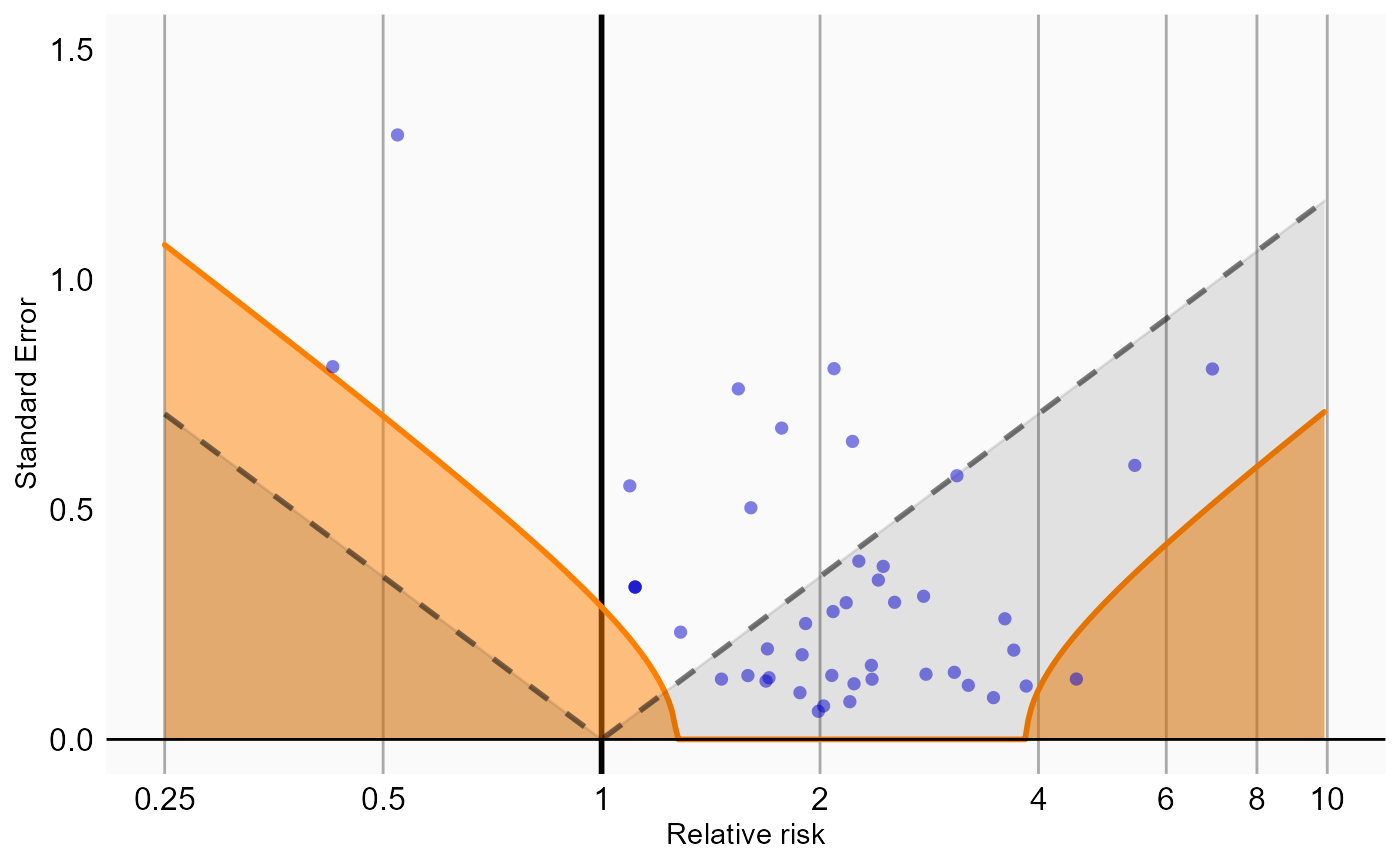
\includegraphics{../inst/doc/EmpiricalPCalibrationVignette_files/figure-latex/unnamed-chunk-7-1.pdf}

In this graph, the blue dots represent the negative controls. Any
estimates below the gray dashed lines will have a traditional p-value
below .05. In contrast, only estimates that fall within the orange areas
will have a calibrated p-value below .05.

\hypertarget{p-value-calibration}{%
\section{P-value calibration}\label{p-value-calibration}}

\hypertarget{calibrating-the-p-value}{%
\subsection{Calibrating the p-value}\label{calibrating-the-p-value}}

We can now use the estimated null distribution to compute the calibrated
p-value for our drug of interest:

\begin{Shaded}
\begin{Highlighting}[]
\NormalTok{p <-}\StringTok{ }\KeywordTok{calibrateP}\NormalTok{(null, drugOfInterest}\OperatorTok{$}\NormalTok{logRr, drugOfInterest}\OperatorTok{$}\NormalTok{seLogRr)}
\NormalTok{p}
\end{Highlighting}
\end{Shaded}

\begin{verbatim}
## [1] 0.8390598
\end{verbatim}

In this case, the calibrated p-value is 0.84, meaning we have very
little confidence we can reject the null hypothesis.

\hypertarget{plotting-the-null-distribution-1}{%
\subsection{Plotting the null
distribution}\label{plotting-the-null-distribution-1}}

A visual representation of the calibration makes it clear why we are no
longer certain we can reject the null hypothesis:

\begin{Shaded}
\begin{Highlighting}[]
\KeywordTok{plotCalibrationEffect}\NormalTok{(negatives}\OperatorTok{$}\NormalTok{logRr,}
\NormalTok{                      negatives}\OperatorTok{$}\NormalTok{seLogRr, }
\NormalTok{                      drugOfInterest}\OperatorTok{$}\NormalTok{logRr, }
\NormalTok{                      drugOfInterest}\OperatorTok{$}\NormalTok{seLogRr, }
\NormalTok{                      null)}
\end{Highlighting}
\end{Shaded}

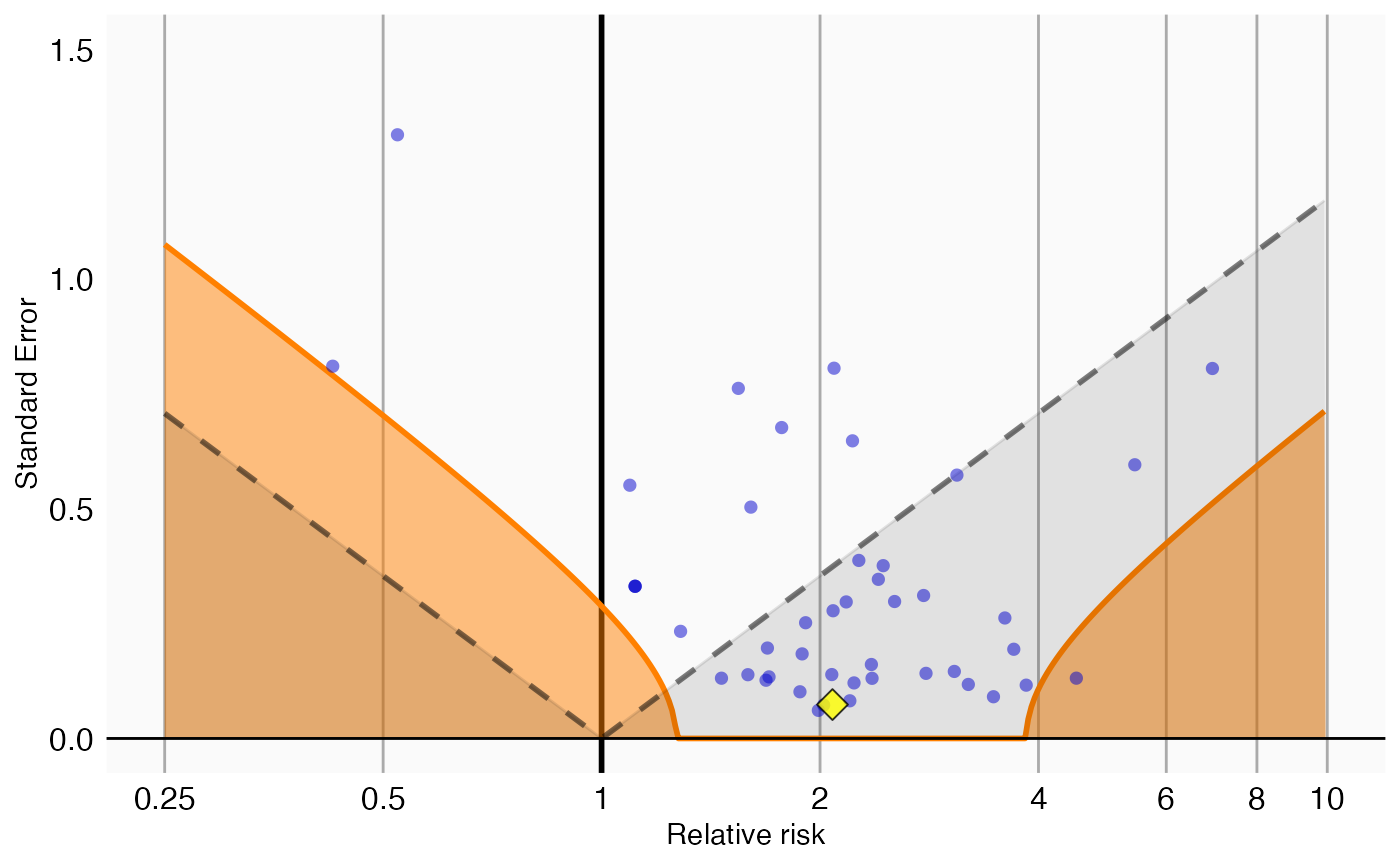
\includegraphics{../inst/doc/EmpiricalPCalibrationVignette_files/figure-latex/unnamed-chunk-9-1.pdf}

In this plot we see that, even though the drug of interest (the yellow
diamond) has a high relative risk, it is indistinguishable from our
negative controls.

\hypertarget{computing-the-credible-interval}{%
\section{Computing the credible
interval}\label{computing-the-credible-interval}}

Depending on how much information we have in terms of number of negative
controls, or precision of those negative controls, we will be more or
less certain about the parameters of the null distribution and therefore
about the calibrated p-value. To estimate our uncertainty we can compute
the 95\% credible interval using Markov Chain Monte Carlo (MCMC). We can
apply the \texttt{fitMcmcNull} function for this purpose:

\begin{Shaded}
\begin{Highlighting}[]
\NormalTok{null <-}\StringTok{ }\KeywordTok{fitMcmcNull}\NormalTok{(negatives}\OperatorTok{$}\NormalTok{logRr, negatives}\OperatorTok{$}\NormalTok{seLogRr)}
\NormalTok{null}
\end{Highlighting}
\end{Shaded}

\begin{verbatim}
## Estimated null distribution (using MCMC)
## 
##           Estimate lower .95 upper .95
## Mean       0.79389   0.67865    0.9056
## Precision 12.79491   6.05934   23.6924
## 
## Acceptance rate: 0.326667333266673
\end{verbatim}

We see that there is uncertainty around the estimates of the mean and
precision (= 1/SD\^{}2), as expressed in the 95\% credible intervals.
This uncertainty can be reduced by either increasing the number of
negative controls, or by increasing the power for the existing controls
(e.g.~by waiting for more data to accumulate).

The acceptance rate of the MCMC seems reasonable (ideal values are
typically between 0.2 and 0.6), but we can investigate the trace just to
be sure:

\begin{Shaded}
\begin{Highlighting}[]
\KeywordTok{plotMcmcTrace}\NormalTok{(null)}
\end{Highlighting}
\end{Shaded}

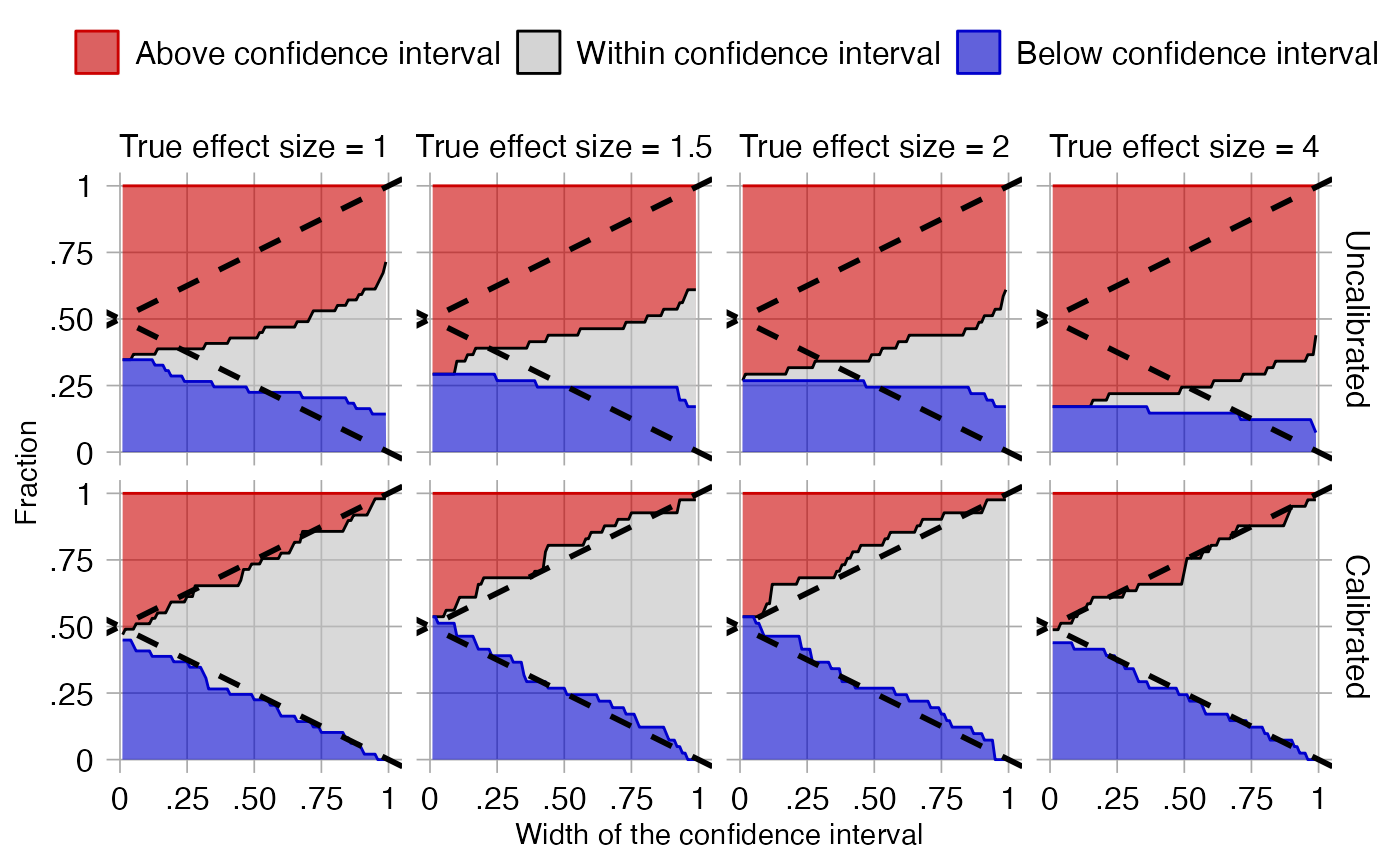
\includegraphics{../inst/doc/EmpiricalPCalibrationVignette_files/figure-latex/unnamed-chunk-11-1.pdf}

For both variables the trace should look like `random noise', as is the
case above. When we see auto-correlation, meaning that one value of the
trace depends on the previous value of the trace, the MCMC might not be
reliable and we should not trust the 95\% credible interval.

We can use the new null object to compute the calibrated p-value as well
as the 95\% credible interval:

\begin{Shaded}
\begin{Highlighting}[]
\NormalTok{p <-}\StringTok{ }\KeywordTok{calibrateP}\NormalTok{(null, drugOfInterest}\OperatorTok{$}\NormalTok{logRr, drugOfInterest}\OperatorTok{$}\NormalTok{seLogRr)}
\NormalTok{p}
\end{Highlighting}
\end{Shaded}

\begin{verbatim}
##           p    lb95ci    ub95ci
## 1 0.8315687 0.5445139 0.9916421
\end{verbatim}

Note that there is uncertainty around the calibrated p-value as
expressed in the 95\% credible interval.

We can also visualize the uncertainty in the p-value calibration by
plotting the 95\% credible interval of the boundary where calibrated p =
0.05, here indicated by the red band:

\begin{Shaded}
\begin{Highlighting}[]
\KeywordTok{plotCalibrationEffect}\NormalTok{(negatives}\OperatorTok{$}\NormalTok{logRr,}
\NormalTok{                      negatives}\OperatorTok{$}\NormalTok{seLogRr, }
\NormalTok{                      drugOfInterest}\OperatorTok{$}\NormalTok{logRr, }
\NormalTok{                      drugOfInterest}\OperatorTok{$}\NormalTok{seLogRr, }
\NormalTok{                      null,}
                      \DataTypeTok{showCis =} \OtherTok{TRUE}\NormalTok{)}
\end{Highlighting}
\end{Shaded}

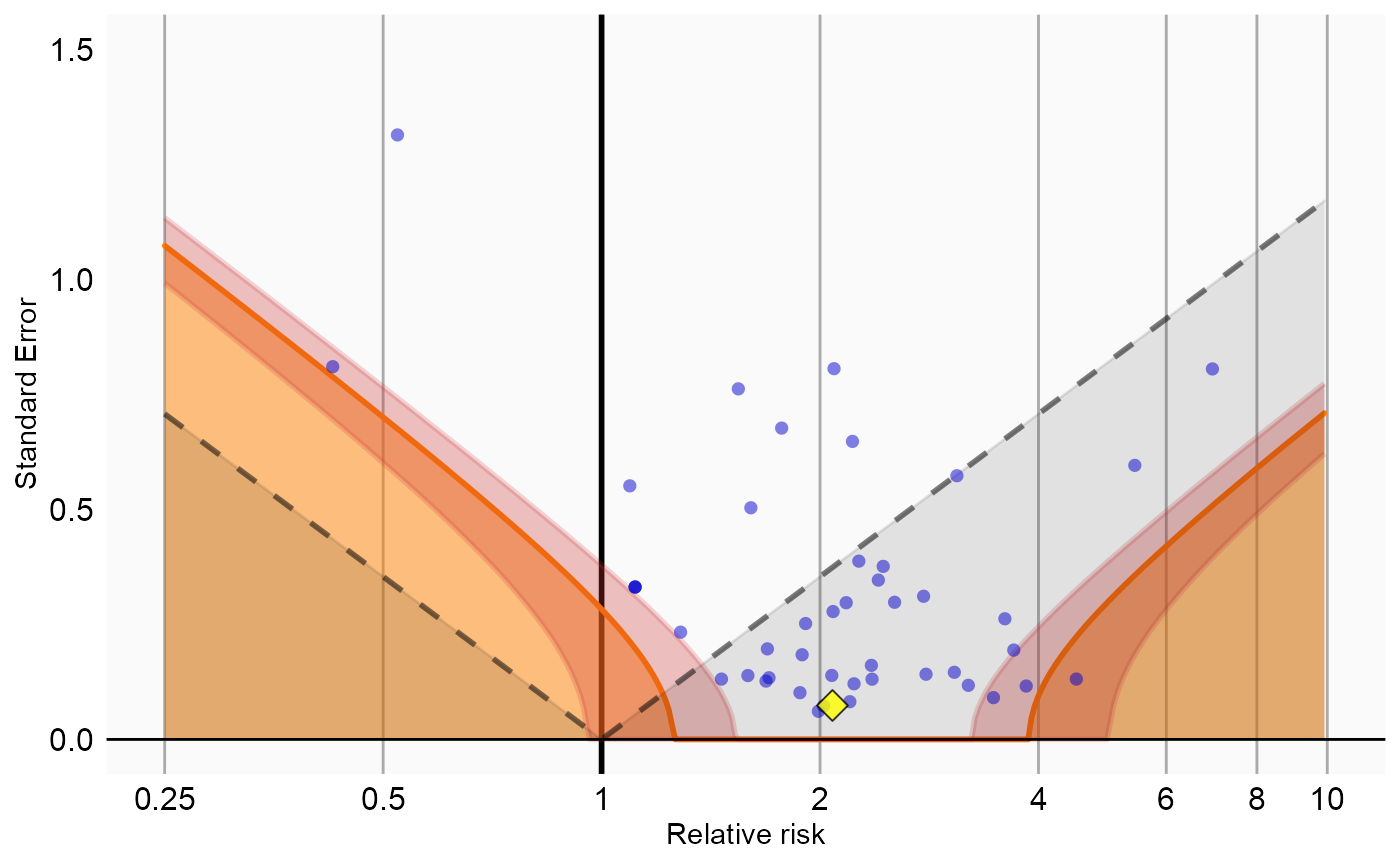
\includegraphics{../inst/doc/EmpiricalPCalibrationVignette_files/figure-latex/unnamed-chunk-13-1.pdf}

\hypertarget{references}{%
\section{References}\label{references}}

\begin{Shaded}
\begin{Highlighting}[]
\KeywordTok{citation}\NormalTok{(}\StringTok{"EmpiricalCalibration"}\NormalTok{)}
\end{Highlighting}
\end{Shaded}

\begin{verbatim}
## 
## To cite EmpiricalCalibration in publications use:
## 
## Schuemie MJ, Ryan PB, DuMouchel W, Suchard MA and Madigan D
## (2014). "Interpreting observational studies: why empirical
## calibration is needed to correct p-values." _Statistics in
## Medicine_, *33*(2), pp. 209-218. <URL:
## http://dx.doi.org/10.1002/sim.5925>.
## 
## Schuemie MJ, Hripcsak G, Ryan PB, Madigan D and Suchard MA (2018).
## "Empirical confidence interval calibration for population-level
## effect estimation studies in observational healthcare data."
## _Proc. Natl. Acad. Sci. U.S.A._, *115*(11), pp. 2571-2577. <URL:
## https://doi.org/10.1073/pnas.1708282114>.
## 
## To see these entries in BibTeX format, use 'print(<citation>,
## bibtex=TRUE)', 'toBibtex(.)', or set
## 'options(citation.bibtex.max=999)'.
\end{verbatim}


\end{document}
